\chapter{Evaluierung der durchgeführten Articulation Work} % (fold)
\label{cha:eval_aw}

Die Evaluierung der durchgeführten „Articulation Work“ bildet den letzten Teil der empirischen Untersuchung und prüft  letztendlich die Eignung des Werkzeugs für den intendierten Verwendungszweck im Sinne der Zielsetzung. Abbildung \ref{fig:img_Kontextgrafiken_k14} stellt dieses Kapitel und dessen Aufbau im Kontext der anderen inhaltlich vor- und nachgelagerten Kapitel dar.


\begin{figure}[htbp]
	\centering
		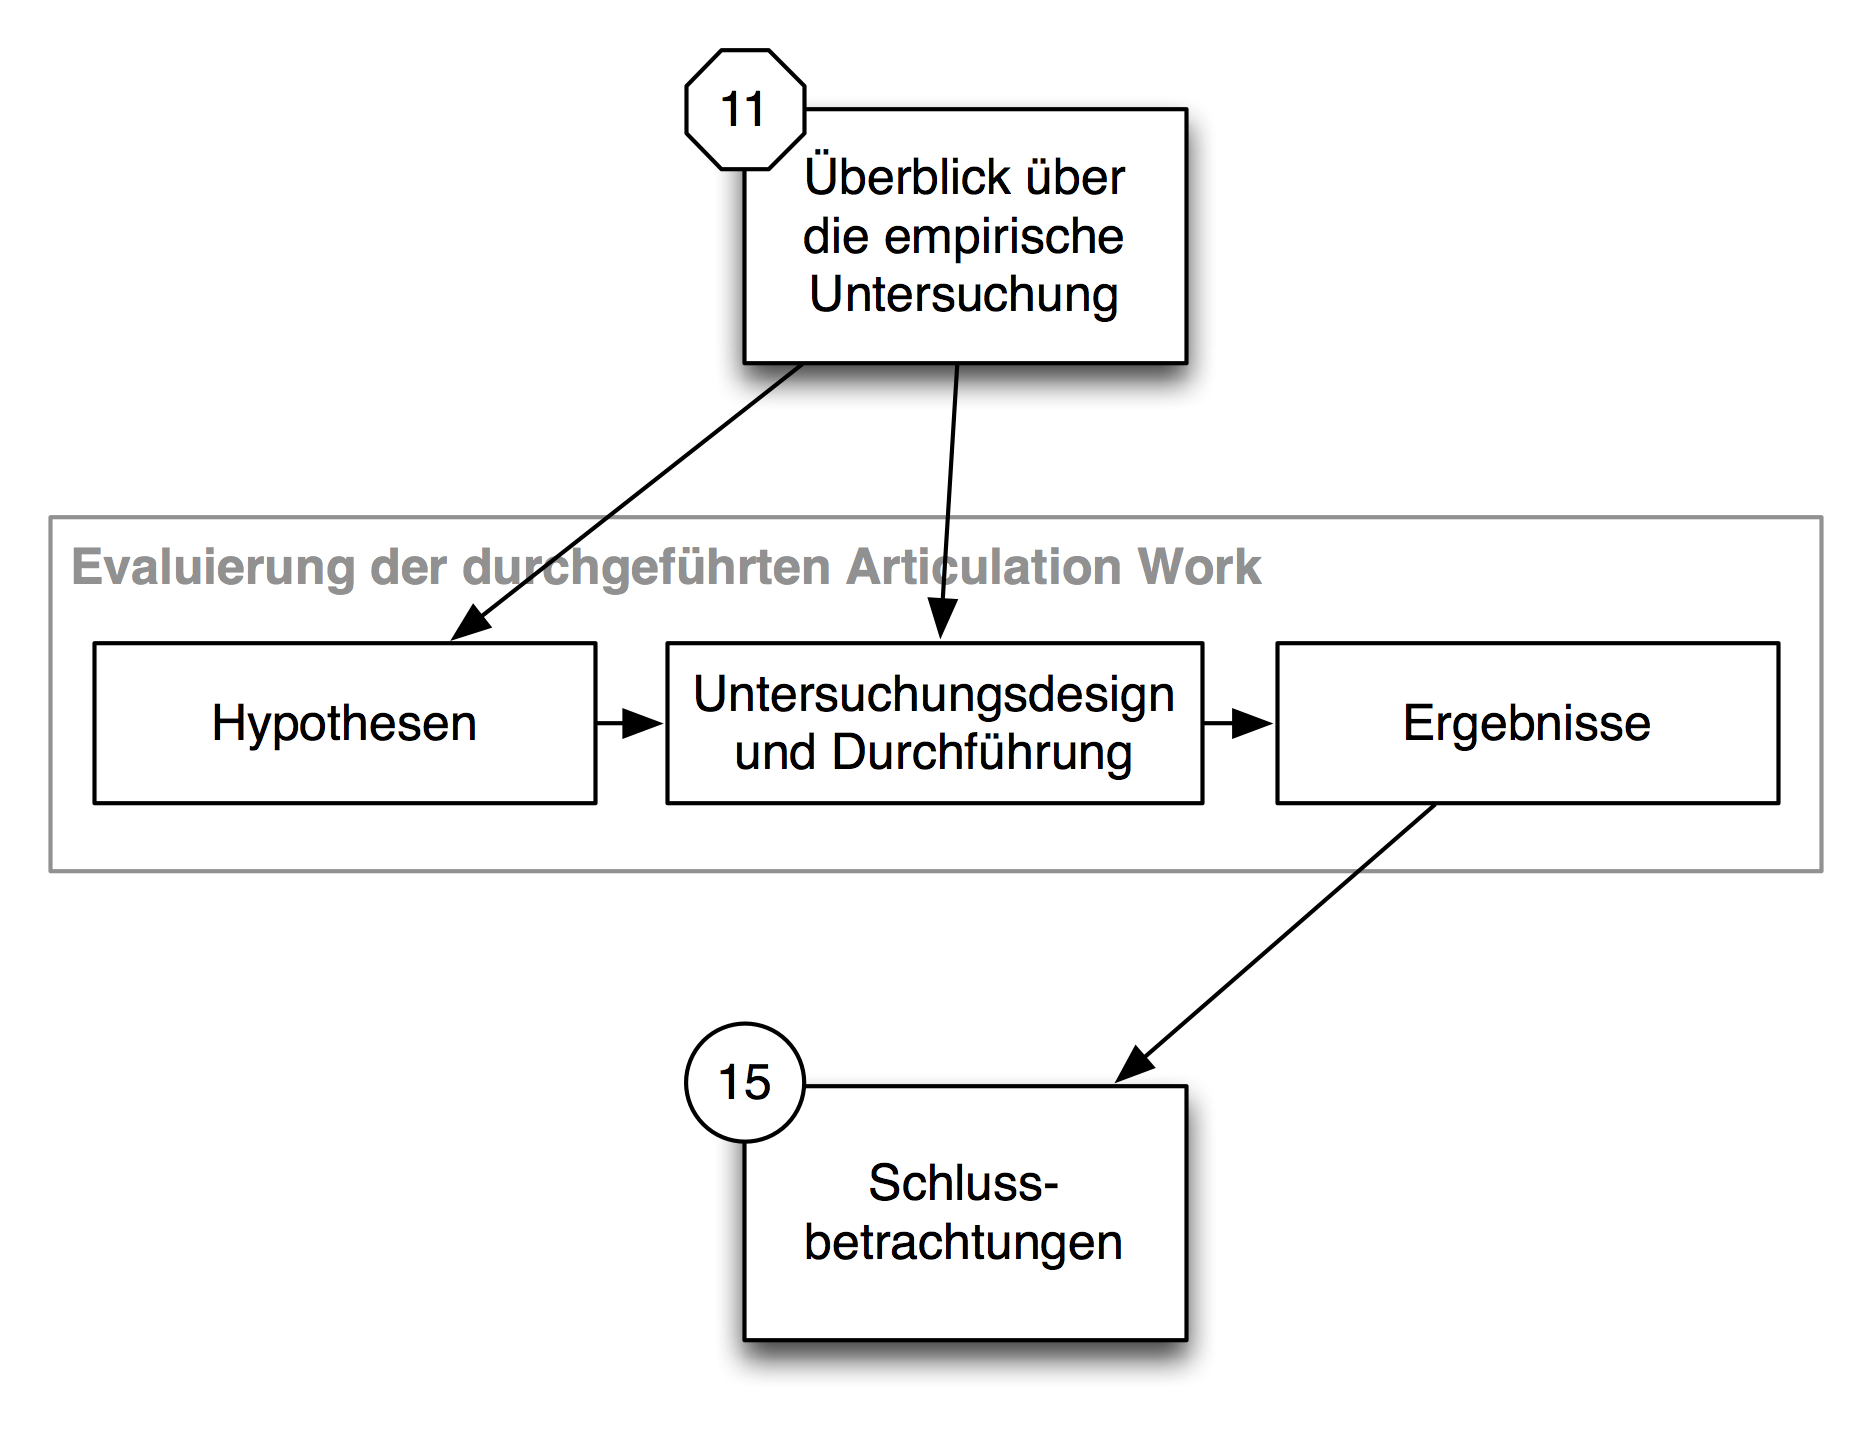
\includegraphics[scale=0.6]{img/Kontextgrafiken/k14.png}
	\caption{Kapitel „Evaluierung der durchgeführten Articulation Work“ im Gesamtzusammenhang}
	\label{fig:img_Kontextgrafiken_k14}
\end{figure}


Die in diesem Kapitel formulierten Hypothese basieren unmittelbar auf der Zielsetzung dieser Arbeit und den in Kapitel \ref{cha:articulation_work} identifizierten Merkmalen erfolgreich durchgeführter „Articulation Work“. Es wird nicht mehr auf die Verwendung der Werkzeugs selbst (siehe Kapitel \ref{cha:eval_werkzeug}) und nicht mehr auf die Rolle von externalisierten Modellen im Kontext dieser Arbeit (siehe Kapitel \ref{cha:eval_modell}) eingegangen.

\section{Hypothesen} % (fold)
\label{sec:a_hypothesen}

In diesem Abschnitt werden die Hypothesen angeführt und begründet, die in diesem Teil der empirischen Untersuchung geprüft werden. Die im Folgenden beschriebenen Hypothesen gehen aber auf die Wirkung von „Articulation Work“ auf die reale Welt ein. Nicht Gegenstand der Untersuchung ist die Verwendung diagrammatischer Modelle zum Zwecke der Durchführung von „Articulation Work“ (siehe \ref{cha:eval_modell}) und die Wirkung des Werkzeugs bei der Durchführung (siehe \ref{cha:eval_werkzeug}).

\subsection{Konzeptuell begründete Hypothesen} % (fold)
\label{sub:a_konzeptionell_begründete_hypothesen}

Die folgenden Hypothesen sind unmittelbar aus der globalen Zielsetzung dieser Arbeit abgeleitet. Die Wirkung von „Articulation Work“ zeigt sich in der organisationalen Realität an der Durchführung der „Production Work“ \citet{Fujimura87}. Um die Wirkung der mit dem Werkzeug durchgeführten „Articulation Work“ zeigen zu können, muss deshalb neben dieser auch die „Production Work“ betrachtet werden. Die Überprüfung erfolgt dabei in zwei Schritten. 

Im ersten Schritt wird die Durchführung der „Articulation Work“ selbst betrachtet. Im Rahmen der Verwendung der Externalisierung von mentalen Modellen zum Zwecke der Durchführung von „Articulation Work“ ist es -- wie in Kapitel \ref{cha:methodik} ausgeführt und in Anforderung \ref{anf:kollaborative_und_unmittelbare_manipulierbarkeit_des_modells} abgebildet -- notwendig, eine kooperative Nutzung des unterstützenden Werkzeugs zu ermöglichen. Ein wesentlicher Schritt zur erfolgreichen Durchführung von „Articulation Work“ ist neben der eigentlichen Externalisierung (die in den ersten beiden Hypothesen des vorhergehenden Kapitels \ref{cha:eval_modell} abgebildet wurde) die Abstimmung der indviduellen mentalen Modelle der Beteiligten. „Abstimmung“ bedeutet hier einen Abgleich der indviduellen Verständnisse jener Arbeitsaspekte, die im Sinne von Kapitel \ref{cha:articulation_work} „problematisch“ sind bzw. enge Kooperation der Beteiligten in der „Production Work“ bedingen. Die Prüfung dieser Hypothese ermöglicht die Beurteilung der Erfüllung der Anforderung \ref{anf:unterstützung_der_iterativen_aushandlung_des_modells} (siehe Seite \pageref{anf:unterstützung_der_iterativen_aushandlung_des_modells}).

\begin{hyp}
	\label{hyp:abstimmung}
	Das Werkzeug unterstützt den Prozess der Abstimmung der individuellen Modelle zwischen Personen.
\end{hyp}

Der zweite Schritt der Untersuchung in diesem Teil der Evaluierung betrachtet letztendlich die durchgeführte Arbeit selbst. Das globale Ziel des hier vorgestellten Ansatzes ist die Unterstützung von Articulation Work. Ob diese tatsächlich erfolgreich durchgeführt wurde, zeigt sich an der Wirkung auf die zugehörige kooperativer Arbeit (die „Production Work“). Es ist also zu beurteilen, ob die Anwendung des Werkzeuges tatsächlich auf die jeweils betrachteten Arbeitsabläufe wirkt und welcher Natur diese Auswirkungen sind. Die Prüfung dieser Hypothese ermöglicht die Beurteilung der Erfüllung der globalen Zielsetzung (siehe Seite \ref{zielsetzung}).

\begin{hyp}
	\label{hyp:wirkung}
	Die Anwendung des Werkzeugs hat Auswirkungen auf die Ergebnisse kooperativer Arbeit.
\end{hyp}

Hinsichtlich der in Kapitel \ref{cha:anforderungen} formulierten Anforderungen können die hier formulierten Hypothesen zusammenfassend wie in Tabelle \ref{tab:hyp_aw} dargestellt eingeordnet werden.

\begin{table}[htbp]
	\centering
	\caption{Hypothesen zu Articulation Work und deren Bezug zu den Anforderungen an das Werkzeug}
\begin{tabular}{|c|c|}
  \hline
   Hypothese & Anforderung \\ \hline
   \ref{hyp:abstimmung} & \ref{anf:unterstützung_der_iterativen_aushandlung_des_modells} \\
   \ref{hyp:wirkung} & globale Zielsetzung \\ \hline
\end{tabular} 
	\label{tab:hyp_aw}
\end{table}

% subsection konzeptionell_begründete_hypothesen (end)

% section hypothesen (end)

\section{Untersuchungsdesign und Durchführung} % (fold)
\label{sec:a_untersuchungsdesign}

In diesem Abschnitt wird auf Basis der oben formulierten Hypothesen das Untersuchungsdesign abgeleitet und die Durchführung der Untersuchung beschrieben. Der erste Teil des Abschnitts beschreibt die Operationalisierung der Hypothesen und damit die Festlegung wie diese konkret geprüft werden können. Im zweiten Teil des Abschnitts wird die Durchführung der Prüfung beschrieben. Hier erfolgt neben der Zuordnung der einzelnen Evaluierungsblöcke (siehe Abschnitt \ref{sec:globales_untersuchungsdesign}) auch die Darstellung rein beschreibender Modell-Parameter, die nicht unmittelbar in die Prüfung der Hypothesen eingehen. 

\subsection{Operationalisierung} % (fold)
\label{sub:a_operationalisierung}

In diesem Abschnitt wird für jede Hypothese identifiziert, in welcher Form sie geprüft werden kann. Dies umfasst die Festlegung der Messpunkte sowie der jeweiligen Mess- und Auswertungsmethode (letztere bezugnehmend auf den in Abschnitt \ref{sec:eingesetzte_werkzeuge_und_verfahren} beschriebenen Verfahren). Zudem werden jene Evaluierungsblöcke festgelegt, die für die jeweilige Untersuchung herangezogen wurden.

Für jede Hypothese wird also spezifiziert, anhand welcher Aspekte diese geprüft werden kann (= abhängige Variablen). Zudem wird festgelegt welche Ausgangssituation bei der Anwendung gewählt werden muss, um die Prüfung durchführen zu können (= unabhängige Variable) und welche Faktoren die Beurteilung ggf. ungewollt beeinflussen können (= Störvariablen).

\subsubsection{Abstimmung individueller Modelle} % (fold)
\label{ssub:abstimmung_individueller_modelle}

Gegenstand dieses Abschnitts ist die Prüfung der Hypothese \ref{hyp:wirkung}. Diese bezieht sich auf die geforderte Eigenschaft des Werkzeugs, den Prozess der Abstimmung der individuellen Modelle zwischen den beteiligten Personen zu unterstützen.

Voraussetzung zur Prüfung dieser Hypothese ist, dass die Aufgabenstellung einem der beiden kooperativen Anwendungsszenarien zuzuordnen ist (siehe Abschnitt \ref{sub:abstimmung_individueller_mentaler_modelle} bzw. \ref{sub:aushandlung_individueller_mentaler_modelle}), in denen alle Teilnehmenden ihrer individuellen mentalen Modelle einbringen. Die Zielsetzung muss so formuliert sein, dass eine gemeinsame Sicht auf den behandelten Sachverhalt angestrebt wird. Weitere Voraussetzungen etwa hinsichtlich der Auswahl der beteiligten Individuen bestehen nicht.

Zur Prüfung, ob eine Abstimmung der individuellen Modelle der beteiligten Personen erreicht wurde, kann auf qualitative Beurteilung durch die Teilnehmenden zurückgegriffen werden. Zur Beurteilung bieten sich hier neben der direkten Frage nach der subjektiv wahrgenommene Abstimmung des Verständnisses auch Teilaspekte des \gls{PMS}-Framework \citep{Sedera02} an, das unter anderem die Wirkung der Modellbildung auf die beteiligten Personen und die Arbeitsrealität abbildet (zur Eignung des \gls{PMS}-Frameworks im Kontext dieser Arbeit siehe \citep{Wahlmuller10}).

Zusätzlich könnte zur Prüfung der Hypothese eine Diagnose der mentalen Modelle der Beteiligten etwa im Sinne von \citep{Ifenthaler06} durchgeführt werden. Hier müssten dann jeweils die externalisierten mentalen Modelle aller Beteiligten jeweils vor und nach dem Abstimmungsprozess gegenübergestellt werden. Die Anwendung dieses Vorgehens übersteigt jedoch den methodischen Fokus dieser Arbeit und wurde in der vorliegenden Untersuchung aus Ressourcengründen nicht durchgeführt.

% subsubsection abstimmung_individueller_modelle (end)

\subsubsection{Auswirkungen auf die Ergebnisse kooperativer Arbeit} % (fold)
\label{ssub:auswirkungen_auf_die_ergebnisse_kooperativer_arbeit}

Gegenstand dieses Abschnitts ist die Prüfung der Hypothese \ref{hyp:keine_einschränkung}. Diese bezieht sich letztendlich auf die Rückwirkung der mit Hilfe des Werkzeugs durchgeführten Aktivitäten auf die Realität.

Voraussetzung zur Prüfung dieser Hypothese ist, dass die Aufgabenstellung einen Sachverhalt zum Gegenstand hat, der eine unmittelbare Entsprechung in der realen (Arbeits-)Welt der Teilnehmenden hat. Weitere Voraussetzungen etwa hinsichtlich der Auswahl der beteiligten Individuen bestehen nicht.

Zur Prüfung dieser Hypothese kann wiederum auf eine qualitative Beurteilung der eingetretenen Veränderungen durch die beteiligten Personen zurückgegriffen werden. Auch hier liefert das \gls{PMS}-Framework \citep{Sedera02} wieder Ansatzpunkte zur Erhebung. Wichtig ist in diesem Zusammenhang die Einhaltung eines angemessenen zeitlichen Abstandes zwischen Modellbildung und Befragung, so dass etwaige Veränderungen in Kraft gesetzt bzw. beobachtete werden können.

Neben der Befragung der teilnehmenden Individuen können auch die Arbeitsabläufe, die Gegenstand der „Articulation Work“ waren, selbst beobachtet werden. Bei bereits etablierten Arbeitsabläufen bietet sich eine Gegenüberstellung der Durchführung der Arbeit vor und nach der Modellbildung an. Bei neu einzurichtenden Arbeitsabläufen steht die Möglichkeit der Gegenüberstellung nicht zur Verfügung. Dementsprechend kann lediglich beurteilt werden, ob die Aushandlung eines gemeinsamen Arbeitsablaufs möglich war. Vergleichend können im zweiten Fall dazu identische Arbeitsabläufe ohne dezidierten Abstimmungsschritt herangezogen werden, wobei als Maß für die Güte der Abstimmung die Anzahl der aufgetretenen Probleme in der Zusammenarbeit während der Durchführung der „Articulation Work“ herangezogen werden kann.

% subsubsection auswirkungen_auf_die_ergebnisse_kooperativer_arbeit (end)
% subsection a_operationalisierung (end)

\subsection{Durchführung} % (fold)
\label{sub:a_durchführung}

Die Durchführung der Untersuchungen zur diesem Teil der Evaluierung wurde in den Evaluierungsblöcken 2 und 4 durchgeführt. In Block 2 waren die Teilnehmenden aufgefordert, ein gemeinsames Vorgehen zur Erstellung einer Seminararbeit auszuhandeln und in einem zweiten, späteren Schritt zu reflektieren und ggf. anzupassen. Diese Schritte waren in den Verlauf der Erstellung der Seminararbeit eingebettet, begleiteten also die „Production Work“, an der der Erfolg der „Articulation Work“ zu messen war. Zur Beurteilung des Erfolgs wurden die Teilnehmenden aufgefordert den Verlauf der Erstellung der Seminararbeit in einem Prozess-Tagebuch zu dokumentieren und dabei besonders auf die Zusammenarbeit mit dem jeweiligen Partner einzugehen. Die Ergebnisse flossen in die Prüfung der Hypothese \ref{hyp:wirkung} ein.

In Block 4 wurden die Teilnehmer unmittelbar nach der Modellbildung und in einem Abstand von 8 Wochen zu den erwarteten bzw. tatsächlich eingetretenen Änderungen der Arbeitspraxis befragt. Die Befragung wurde mittels einem auf Basis des \gls{PMS}-Framework erstellten Fragebogen (siehe Anhang \ref{cha:daten_der_empirischen_untersuchung}) durchgeführt. Die Ergebnisse flossen in die Prüfung der Hypothesen \ref{hyp:abstimmung} und \ref{hyp:wirkung} ein.

In diesem Teil der Evaluierung wurden keine deskriptiven Parameter erhoben, weshalb die in den Kapiteln \ref{cha:eval_werkzeug} und \ref{cha:eval_modell} an dieser Stelle vorgenommene Beschreibung derselben hier entfällt.

\subsubsection{Stichprobe} % (fold)

Für die Untersuchung der Hypothesen in diesem Kapitel wurden die Evaluierungsblöcke 1 bis 5 herangezogen. Die Stichprobe setzt sich wie in Tabelle \ref{tab:stichprobe_aw} beschrieben zusammen.

\begin{table}[htbp]
	\centering
	\caption{Stichproben der Evaluierung zur Articulation Work}

		\begin{tabular}{| l || c | c |}
		\hline
			Evaluierungsblock & $n_{Anwendungen}$ & $n_{Teilnehmende}$ \\ \hline
			technische Evaluierung		  &  9 & 18 \\
			Aushandlung 1 (1. Durchgang)  &  9 & 19 \\
			Aushandlung 1 (2. Durchgang)  &  9 & 18 \\
			Concept Mapping 1			  & 18 & 54 \\
			Aushandlung 2				  & 10 & 13 \\
			Concept Mapping 2 (Tisch)     & 11 & 24 \\
			Concept Mapping 2 (CMapTools) & 12 & 25 \\ \hline
			Gesamt						  & 78 & 171 \\ \hline
	\end{tabular}
	\label{tab:stichprobe_aw}
\end{table}
% subsubsection stichprobe (end)

% subsection a_durchführung (end)
% section untersuchungsdesign (end)

\section{Ergebnisse} % (fold)
\label{sec:a_ergebnisse}

In diesem Abschnitt werden die Ergebnisse der Untersuchung gegliedert nach den oben formulierten Hypothesen dargestellt. Zu jeder Hypothese wird die Auswertung der empirischen Daten dargestellt, die Bedeutung der empirischen Belege für die Prüfung der jeweiligen Hypothese diskutiert und letztendlich das Ergebnis zusammenfassend dargestellt.  

\subsection{Abstimmung individueller Modelle} % (fold)
\label{sub:abstimmung_individueller_modelle}

Gegenstand der hier beschriebenen Untersuchung ist Hypothese \ref{hyp:abstimmung} („Das Werkzeug unterstützt den Prozess der Abstimmung der individuellen Modelle zwischen Personen.“). Als Grundlage dieser Untersuchung dienen die Ergebnisse der Evaluierungsblöcke 2 und 4.

\subsubsection{Auswertung} 

\subsubsection{Diskussion} 

\subsubsection{Ergebnis} 

% subsection abstimmung_individueller_modelle (end)

\subsection{Auswirkungen auf die Ergebnisse kooperativer Arbeit} % (fold)
\label{sub:auswirkungen_auf_die_ergebnisse_kooperativer_arbeit}

Gegenstand der hier beschriebenen Untersuchung ist Hypothese \ref{hyp:wirkung} („Die Anwendung des Werkzeugs hat Auswirkungen auf die Ergebnisse kooperativer Arbeit.“). Als Grundlage dieser Untersuchung dienen die Ergebnisse der Evaluierungsblöcke 2 und 4.

\subsubsection{Auswertung} 

\subsubsection{Diskussion} 

\subsubsection{Ergebnis} 

% subsection auswirkungen_auf_die_ergebnisse_kooperativer_arbeit (end)
% section ergebnisse (end)

\section{Zusammenfassung} % (fold)
\label{sec:a_zusammenfassung}

% section zusammenfassung (end)
% chapter eval_aw (end)